%!TEX root = ../Thesis.tex
%Notes:symmetrically arranged, neglect the drag created by the frame,
In this chapter, the notations and reference frames used in the assignment will be stated. Methods to transfer between coordinate frames will also be examined. Furthermore, a dynamic model of a quadrotor UAV is developed. A representation of the system is useful for simulations, deriving state estimators and for controller design. In this assignment, the following assumptions have been made: The quadcoper is assumed to be symmetric, in other words, all the motors and propellers are equally sized and the lever from the quadcoper center to the motors have the same lengths. Moreover, the multirotor is assumed to have a rigid body, the mass of the propellers is approximated to zero and that the drag force due to air resistance is negligible.

The quad-rotor UAV has been a popular platform due to its simplicity. By using four variable speed motors with fixed pitch propellers, the UAV gets a simple mechanical structure that makes the UAV fully controllable. A god approximation of the force from the propellers is stated in equation \ref{eq:propForce}.
\begin{equation}\label{eq:propForce}
  f=k\omega^{2}
\end{equation}
Where $k>0$ is a constant depending on the shape of the propeller, gear ratio and density of air. $\omega$ is the angular velocity of the motor (\cite{lozano2013unmanned}). This chapter is based on the feasibility study written by the author \citep{Line2017}.

\section{Notation}\label{sec:notation}
The notations used in this assignment are mainly based on the notations used in \cite{Fossen2011}. A coordinate free vector is written as $\vec{u}$. To write a vector relative to coordinate system \{n\}, the notation $\vect{u}^{n}$ is used. When a point is differentiated, it must be done with respect to a reference frame. The notation used for describing this is the subscript $u_{obj/ref}$. For example, the velocity of a particle in reference frame \{a\} relative to reference frame \{b\} given in frame \{c\} is written as $v^{c}_{a/b}$. Vectors are written as lowercase letters, while matrices are written as uppercase. The inverse of a matrix or vector is written as $\vect{A}^{-1}$ and $\vect{A}^\top$ as the transpose.

\section{Reference Frames}\label{sec:refFrame}
To be able to derive system equations for a vehicle in motion, several reference frames needs to be established. An overview of the reference frames used in this assignment are summarized in table \ref{tab:refFrames}. Where the Body frame is fixed to the frame of the UAV, where it is often placed in the the UAV center as illustrated in figure \ref{fig:quadRef}. The ECI frame is centered in the Earths mass center and is fixed in space, unlike the ECEF frame which is also centered in the Earths mass center but is rotating with the Earth (\cite{Fossen2011}). Both the ECI and ECEF have their $z$ axis pointing along with the Earth's rotation axis (\cite{vik2009integrated}). The NED frame is in this assignment defined as a fixed frame located at a tangent plane at the Earth's reference ellipsoid close to the UAV. The NED frame's $x$ axis is pointing towards true North, the $y$ axis is pointing towards East and the resulting $z$ frame points downwards normal to the ellipsoid. ENU frame is often used as an alternative to the NED frame. The $x$, $y$ and $z$ axis of the ENU frame is pointing in the East, North and upwards normal to the ellipsoid respectively. The CG frame is placed in the center of gravity of the vehicle, and is orientated at the same direction as the Body frame (\cite{Fossen2011}).

\begin{table}[!htb]
  \centering
  \begin{tabular}{l l l}
    \toprule
    Name&Description&Symbol\\ \hline
    Body&Body-fixed reference&$b$\\
    CG&Center of gravity&$g$\\
    ECEF&Earth-centered Earth fixed&$f$\\ %(GNSS)
    ECI&Earth-centered inertial&$i$\\
    NED&North-East-Down&$n$\\
    ENU&East-North-Up&$e$\\
    GEO&Geodetic Coordinate System&$ge$\\
    \bottomrule
  \end{tabular}
  \caption{Reference frames}
  \label{tab:refFrames}
\end{table}

\section{Euler angles}\label{sec:euler}
The attitude of the Body frame relative to NED is often given by the Euler angles $\vect{\Theta}_{nb}=[\phi, \; \theta, \; \psi]^\top$ (\cite{Fossen2011}). The Euler angles geometrical definition is given in figure \ref{fig:Eulerangles}, where $\phi$, $\theta$ and $\psi$ are often referred to as roll, pitch and yaw respectively.
\begin{figure}[!htp]
  \begin{minipage}[b]{0.5\linewidth}
    \centering
    \def\svgwidth{\linewidth}%{0.70}
    \import{img/}{zyx_convention.pdf_tex}
    \caption{Geometrical definition of Euler angles}
    \label{fig:Eulerangles}
  \end{minipage}
  \hspace{0.5cm}
  \begin{minipage}[b]{0.5\linewidth}
    \centering
    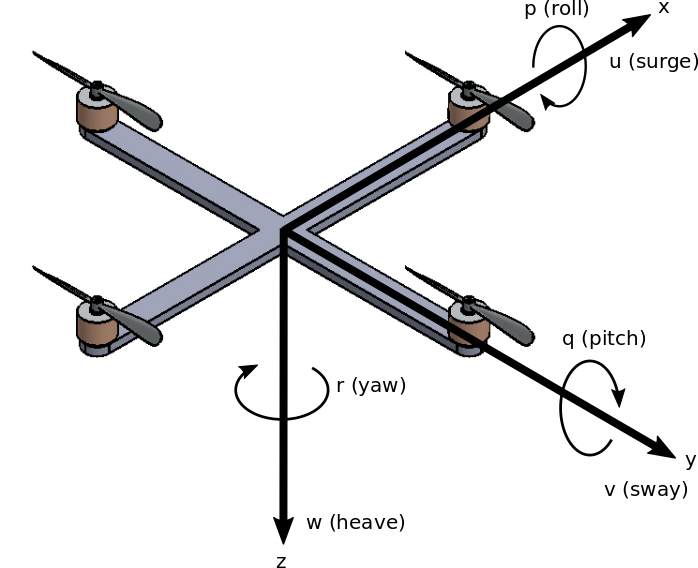
\includegraphics[width=\linewidth]{img/simpleQuadEuler.png}
    \caption{Linear velocities $u$,$v$,$w$ and the angular velocities $p$, $q$, $r$}{The linear velocities $u$,$v$,$w$ and the angular velocities $p$, $q$, $r$. All given in Body frame}
    \label{fig:quadEuler}
  \end{minipage}
\end{figure}

Transformation of a vector $\in \R^3$ given in the body frame $b$ to the NED frame $n$ is often performed using a rotation matrix $\vect{R}_b^n(\vect{\Theta_{nb}})$. As figure~\ref{fig:Eulerangles} illustrates, this assignment uses the $zyx$ convention. In other words, the rotational transformation is performed by first rotate an angle $\psi$ about the $z$ axis, followed by the rotation $\theta$ about the $y$ axis and finally rotate $\phi$ about the $x$ axis. The transformation matrix $\vect{R}_b^n$ in $zyx$ convention as a function of $\vect{\Theta_{nb}}$ is then given as (\cite{Fossen2011}).
\begin{equation}\label{eq:rotMat}
\vect{R}_b^n(\vect{\Theta_{nb}})=
  \begin{bmatrix}
    c_\psi c_\theta & -s_\psi c_\phi+c_\psi s_\theta s_\phi & s_\psi s_\phi+c_\psi s_\theta c_\phi\\
    s_\psi c_\theta & c_\psi c_\phi+s_\phi s_\theta s_\psi & -c_\psi s_\phi+s_\psi s_\theta c_\phi\\
    -s_\theta & c_\theta s_\phi & c_\theta c_\phi
  \end{bmatrix}
\end{equation}
where $c_x$ and $s_x$ is abbreviations for $\cos(x)$ and $\sin(x)$ respectively. The rotational transformation from NED to body, can be found by taking the inverse of \ref{eq:rotMot} \citep{Fossen2011}.
\begin{equation}
  \vect{R}_n^b(\vect{\Theta_{nb}})=\vect{R}_b^n(\vect{\Theta_{nb}})^{-1}
\end{equation}

Due to the inconsistent use of the reference frames NED and ENU, a method to transfer between thees two frames needs to be established. The attitude of the ENU frame relative to the NED frame can be given as the Euler angles $\vect{\Theta}_{ne}=[\pi,0,\pi/2]^{\top}$. By using the rotation matrix given in \ref{eq:rotMat}, the rotational transformation from NED to ENU can be given as
\begin{equation}\label{eq:rotMatENU2NED}
  \vect{R}_e^n(\vect{\Theta_{ne}})=
  \begin{bmatrix}
    0 & 1 & 0\\
    1 & 0 & 0\\
    0 & 0 & -1
  \end{bmatrix}
\end{equation}
Due to the symmetry of the matrix, we get that $\vect{R}_e^n(\vect{\Theta_{ne}})=\vect{R}_n^e(\vect{\Theta_{ne}})$.

The angular velocity transformation from the body-fixed angular velocities to the Euler rate vector can be given as (\cite{Fossen2011})
\begin{equation}
  \vect{\dot{\Theta}}_{nb}=\vect{T}_\Theta(\vect{\Theta}_{nb})\vect{\omega}^b_{b/n}
\end{equation}
Where $\vect{T}_\Theta(\vect{\Theta}_{nb})$ is
\begin{equation}
\vect{T}_\Theta(\vect{\Theta}_{nb})=
  \begin{bmatrix}
    1&s_\phi t_\theta & c_\phi t_\theta\\
    0 & c_\phi & -s_\phi\\
    0 & s_\phi/c_\theta & c_\phi/c_\theta
  \end{bmatrix}
\end{equation}
in this matrix, $s_x$, $c_x$ and $t_x$ is abbreviations for $\sin(x)$, $\cos(x)$ and $\tan(x)$ respectively.

\section{Unit Quaternions}\label{sec:quat}
Unit quaternions is an alternative to the Euler-angle representation described in \ref{sec:euler}. This four parametric representation of a rotation 
has the benefit of being able to represent singularity-free three dimensional rotations (\cite{Fossen2011}). A quaternion $\vect{q}$ is defined as:
\begin{equation}
  \vect{q}=
  \begin{bmatrix}
    \eta\\
    \epsilon_1\\
    \epsilon_2\\
    \epsilon_3
  \end{bmatrix}
  =
  \begin{bmatrix}
    \eta\\
    \vect{\epsilon}
  \end{bmatrix}
\end{equation}
where $\eta$ is the real part and $\vect{\epsilon}$ is the complex part of the quaternion. In addition, the unit quaternions must satisfy the following constraint (\cite{Fossen2011})
\begin{equation}
  \vect{q}^\top\vect{q}=1
\end{equation}


The angular velocity of a unit quaternion can be derived as
\begin{equation}
  \vect{\dot{q}}=
  \begin{bmatrix}
    \dot{\eta}\\
    \vect{\dot{\epsilon}}
  \end{bmatrix}
  =\frac{1}{2}
  \begin{bmatrix}
    -\vect{\epsilon}^\top\\
    \eta \vect{I}^{3 \times 3}+\vect{S(\epsilon)}
  \end{bmatrix}
  \vect{\omega}_{b/n}^{b}
\end{equation}
Furthermore, the rotation matrix for unit quaternions from coordinate frame a to b is states as (\cite{Fossen2011})
\begin{equation}\label{eq:rotMatQua}
\vect{R}(\vect{q})_a^b=
  \begin{bmatrix}
    1-2(\epsilon_2^2+\epsilon_3^2) & 2(\epsilon_1 \epsilon_2 -\epsilon_3 \eta) & 2(\epsilon_1 \epsilon_3 + \epsilon_2 \eta)\\
    2(\epsilon_1 \epsilon_2 + \epsilon_3 \eta) & 1-2(\epsilon_1^2+\epsilon_3^2) & 2(\epsilon_2 \epsilon_3 - \epsilon_1 \eta)\\
    1(\epsilon_1 \epsilon_3 - \epsilon_2 \eta) & 2(\epsilon_2 \epsilon_3 + \epsilon_1 \eta) & 1-2(\epsilon_1^2+\epsilon_2^2)
  \end{bmatrix}
\end{equation}

As in the Euler angles notation in \ref{sec:euler}, there is also an angular velocity transformation for unit quaternions (\cite{Fossen2011})
\begin{equation}
  \vect{\dot{q}}=\vect{T}_q(\vect{q})\vect{\omega}^b_{b/n}
\end{equation}
Where $\vect{T}_q(\vect{q})$ is
\begin{equation}
\vect{T}_q(\vect{q})=
  \begin{bmatrix}
    -\epsilon_1 & -\epsilon_2 & -\epsilon_3\\
    \eta & -\epsilon_3 & \epsilon_2\\
    \epsilon_3 & \eta & -\epsilon_1\\
    -\epsilon_2 & \epsilon_1 & \eta
  \end{bmatrix}
\end{equation}

Converting Euler angles to quaternions and the other way around can be done by requiring the that the rotation matrices for both Euler-angles and unit quaternions are equal (\cite{vik2009integrated}).
\begin{equation}
  \vect{R}(\vect{q})_a^b=\vect{R}(\vect{\Theta})_a^b
\end{equation}

\section{Geodetic coordinates} % (fold)
\label{sub:geodetic_coordinates}
One method to represent a global position near the surface of the earth is by using the geodetic coordinate system. Geodetic coordinate systems depends on a reference ellipsoid of the earth. The coordinate system describes the position of a point with the variables longitude, latitude and height respectively denoted as $\lambda$, $\phi$ and $h$. Where the longitude is the rotational angle between the Prime Median and the point, latitude is the angle between the equator plane and the normal of the reference ellipsoid passing trough the point and height is the distance between the ellipsoid and the point \citep{cai2011unmanned}.

All GNSS receivers used in this assignment refers to the same WGS-84 ellipsoid model. \cite{cai2011unmanned} summarize the WGS-84 parameters as
\begin{align}
  R_{Ea}&=6378137.0m\\
  f&=1/298.257223563
\end{align}
where $R_{Ea}$ is the semi-major axis and $f$ is the flattering factor. Further on, the semi-minor axis $R_{Eb}$, first eccentricity $e$, median radius of curvature $M_E$ and the prime vertical radius of curvature $N_E$ are defined as
\begin{align}
  R_{Eb}&=R_{Ea}(1-f)\\
  e&=\frac{\sqrt{R_{Ea}^2-R_{Eb}^2}}{R_{Ea}}\\
  M_e&=\frac{R_{Ea}(1-e^2)}{(1-e^2\sin^2{\phi})^{3/2}}\\
  N_E&=\frac{R_{Ea}}{\sqrt{1-e^2\sin^2{\phi}}}
\end{align}

A point $\vect{p}^{ge}=[\lambda, \phi, h]^{\top}$ in the geodetic coordinate system can be given in the ECEF coordinate system by using the conversion method
\begin{equation}
  \vect{p}^f=
  \begin{bmatrix}
    (N_E+h)\cos{\phi}\cos{\lambda}\\
    (N_E+h)\cos{\phi}\sin{\lambda}\\
    [N_E(1-e^2)+h]\sin{\phi}\\
  \end{bmatrix}\label{eq:ge_to_f}
\end{equation}
\citep{cai2011unmanned}


Furthermore, the point $\vect{p}$ can be represented relative to a local NED coordinate system. In this assignment, the local NED frame $\vect{p}_{loc}$ is defined to be whatever the UAV reads from the GNSS sensor when the \gls{UAV} arms the motors. Equation~\ref{eq:ECEF2NED} states the position conversion given in \cite{cai2011unmanned}
\begin{equation}\label{eq:ECEF2NED}
  \vect{p}^n=\vect{R}_{f}^n(\vect{p}^{ge}_{loc})(\vect{p}^f-\vect{p}_{loc}^f)
\end{equation}
where $\vect{R}_{f}^n(\vect{p}^{ge}_{loc})$ is the rotation matrix from ECEF to the loc NED given as
\begin{equation}
  \vect{R}_{f}^n(\vect{p}^{ge}_{loc})=
  \begin{bmatrix}
    -s_{\phi_{loc}}c_{\lambda_{loc}} & -s_{\phi_{loc}}s_{\lambda_{loc}} & c_{\phi_{loc}}\\
    -s_{\lambda_{loc}} & c_{\lambda_{loc}} & 0\\
    -c_{\phi_{loc}}c_{\lambda_{loc}} & -c_{\phi_{loc}}s_{\lambda_{loc}} & -s_{\phi_{loc}}
  \end{bmatrix}
\end{equation}
where $c_x$ and $s_x$ is abbreviations for $\cos(x)$ and $\sin(x)$ respectively.
% subsection geodetic_coordinates (end)


\section{Skew Symmetric Matrix}\label{sec:skew}
A matrix is said to be skew symmetric if and only if $\vect{S}=\vect{S^\top}$ (\cite{spong2006robot}). The $3\times3$ skew symmetric matrix can be stated as:
\begin{equation*}
\vect{S}(\vect{x})=
  \begin{bmatrix}
    0 & -x_{3} & x_{2}\\
    x_{3} & 0 & -x_{1}\\
    -x_{2} & x_{1} & 0
  \end{bmatrix}
\end{equation*}
where $\vect{x} \in \R^3$. This matrix is useful for performing the vector cross product defined by: (\cite{Fossen2011})
\begin{equation*}
  \vect{a} \times \vect{b} := \vect{S}(\vect{a})\vect{b}
\end{equation*}
where $\vect{a}, \vect{b} \in \R^3$.


\section{Dynamic Modeling of a Quad-Rotor}\label{sec:dynMod}
In this section, the dynamic model for a rigid body quadcoper will be derived using the Newton-Euler approach. Euler's equation can for linear- ($\vec{p}_g$) and angular momentum ($\vec{h}_g$) is 
defined as in equation \ref{eq:eulerEq1} and \ref{eq:eulerEq2} respectively (\cite{Fossen2011}).
\begin{align}\label{eq:eulerEq1}
  \frac{~^n\!d}{dt}\vec{p}_{g}&=\vec{f}_{g} & \vec{p}_{g}&=m\vec{v}_{g/n}
\end{align}
\begin{align}\label{eq:eulerEq2}
  \frac{~^n\!d}{dt}\vec{h}_{g}&=\vec{m}_{g} & \vec{h}_{g}&=I_{g}\vec{\omega}_{b/n}
\end{align}
where $\vec{f}_{g}$ is the force acting on the vehicle, $\vec{m}_g$ is the moment acting on the same rigid body, $m$ is the total mass, $I_g$ is the inertia about the center of gravity, $\vec{v}_{g/n}$
and $\vec{\omega}_{b/n}$ is the linear and angular velocities respectively.

The equation for linear momentum in \ref{eq:eulerEq1} can be rewritten as
\begin{equation}
  \vec{f}_{g}=m\frac{~^n\!d}{dt}\vec{v}_{g/n}
\end{equation}
, and by expressing the equations in body frame the following is obtained:
\begin{align}
  \vec{f}_{g}&=m(\frac{~^b\!d}{dt}\vec{v}_{g/n}+\vec{\omega_{b/n}}\times\vec{v_{b/n}})\\
  \vect{f}_{g}^{b}&=m(\vect{\dot{v}}_{g/n}^{b}+\vect{S}(\vect{\omega}_{b/n}^{b})\vect{v}_{g/n}^{b}) \label{eq:linMot}
\end{align}

Equation \ref{eq:eulerEq2} can be reformulated such that the rotational motion about CG can be expressed in Body frame as
\begin{equation}\label{eq:rotMot}
  \vect{m}_{g}^{b}=\vect{I}_g(\vect{\dot{\omega}}_{b/n}^{b}-\vect{S}(\vect{\omega_{b/n}^{b}})\vect{\omega_{b/n}^{b}})
\end{equation}
where $\vect{S}$ is the skew symmetric matrix defined in \ref{sec:skew}.

Resulting Newton Euler equations from \ref{eq:linMot} and \ref{eq:rotMot} can be written as (\cite{Fossen2011})
\begin{equation}\label{eq:dynFull}
  \begin{bmatrix}
    m\vect{I}^{3 \times 3} & \vect{0}^{3 \times 3}\\
    \vect{0}^{3 \times 3} & \vect{I}_{g}
  \end{bmatrix}	
  \begin{bmatrix}
    \vect{\dot{v}}_{g/n}^{b}\\
    \vect{\dot{\omega}}_{g/n}^{b}
  \end{bmatrix}
  +
  \begin{bmatrix}
    mS(\vect{\omega}_{b}^{b/n}) & \vect{0}^{3 \times 3}\\
    \vect{0}^{3 \times 3} & -\vect{S}(\vect{\omega}_{b}^{b/n})
  \end{bmatrix}
  \begin{bmatrix}
    \vect{v}_{g/n}^{b}\\
    \vect{\omega}_{g/n}^{b}
  \end{bmatrix}
  =
  \begin{bmatrix}
    \vect{f}_{g}^{b}\\
    \vect{m}_{g}^{b}
  \end{bmatrix}
\end{equation}
where $\vect{I}^{3 \times 3}$ is the $3\times3$ identity matrix and $\vect{0}^{3 \times 3}$ is a $3\times3$ matrix containing only zeros. 
The matrix involving the system inertia constants can be states as $\vect{M}_{RB}^{CG}$ and the matrix containing the Coriolis-Centripetal parameters as $\vect{C}_{RB}^{CG}$. Further on, 
the equation \ref{eq:dynFull} can be written in the compact matrix form (\cite{Fossen2011})
\begin{equation}\label{eq:dynCg}
  \vect{M}_{RB}^{CG}
  \begin{bmatrix}
    \vect{\dot{v}}_{g/n}^{b}\\
    \vect{\dot{\omega}}_{g/n}^{b}
  \end{bmatrix}
  +\vect{C}_{RB}^{CG}
  \begin{bmatrix}
    \vect{v}_{g/n}^{b}\\
    \vect{\omega}_{g/n}^{b}
  \end{bmatrix}
  =
  \begin{bmatrix}
    \vect{f}_{g}^{b}\\
    \vect{m}_{g}^{b}
  \end{bmatrix}
\end{equation}
where $\vect{M}_{RB}^{CG}$ is unique, while there is possible to find a large number of representations for $\vect{C}_{RB}^{CG}$ (\cite{Fossen2011}). 

System equations given in \ref{eq:dynCg} are expressed for system motions relative to center of gravity. A more suitable set of equations would be to have the system motions described about a chosen body frame.
A vector $\vect{r}_g^b$ describes the translation from center of gravity to the body frame. By using coordinate transformation, we can according to \cite{Fossen2011} rewrite \ref{eq:dynCg} as
\begin{equation}
  \begin{bmatrix}
    m\vect{I}^{3 \times 3} & -mS(\vect{r}_g^b)\\
    mS(\vect{r}_g^b) & \vect{I}_{b}
  \end{bmatrix}	
  \begin{bmatrix}
    \vect{\dot{v}}_{b/n}^{b}\\
    \vect{\dot{\omega}}_{b/n}^{b}
  \end{bmatrix}
  +
  \begin{bmatrix}
    mS(\vect{\omega}^{b}_{b/n}) & -mS(\vect{\omega}^{b}_{b/n})\vect{S}(\vect{r}_{g}^{b})\\
    -mS(\vect{r}_{g}^{b})\vect{S}(\vect{\omega}^{b}_{b/n}) & -\vect{S}(\vect{I}_{b}\vect{\omega}^{b}_{b/n})
  \end{bmatrix}	
  \begin{bmatrix}
    \vect{v}_{b/n}^{b}\\
    \vect{\omega}_{b/n}^{b}
  \end{bmatrix}
  =
  \begin{bmatrix}
    \vect{f}_{b}^{b}\\
    \vect{m}_{b}^{b}
  \end{bmatrix}
\end{equation}
which again, can be written more compact(\cite{Fossen2011}).
\begin{equation}
  \vect{M}_{RB}\dot{\vect{\nu}}+\vect{C}_{RB}(\vect{\nu})\vect{\nu}=\vect{\tau}_{RB}
\end{equation}
Where $\vect{M}_{RB}$ is often referred to as the Rigid-Body System Inertia Matrix while $\vect{C}_{RB}$ is called Coriolis-Centripetal Matrix. $\vect{\nu}$ is the state vector and $\vect{\tau}_{RB}$ is a generalized vector of 
external forces and moments, both written out in \ref{eq:allStates}.
\begin{align}\label{eq:allStates}
  \vect{\nu}=
  \begin{bmatrix}
    \vect{v}_{b/n}^{b}\\
    \vect{\omega}_{b/n}^{b}
  \end{bmatrix}
  =
  \begin{bmatrix}
    u\\
    v\\
    w\\
    p\\
    q\\
    r
  \end{bmatrix}
  &&
  \vect{\tau}_{RB}=
  \begin{bmatrix}
    \vect{f}_{b}^{b}\\
    \vect{m}_{b}^{b}
  \end{bmatrix}
  =
  \begin{bmatrix}
    X\\
    Y\\
    Z\\
    K\\
    M\\
    N
  \end{bmatrix}
\end{align}

There are two main linear forces acting on the quadcopter. The gravitational force and the force given by the propellers.
For the model developed in this assignment, we approximate the gravitational force to be parallel to the NED frame's z axis. The force due to gravitation is then given as $\vect{f}_{g,g}^{n}=mg [0\,0\,1]^T$. By transferring this force to
body frame, the gravitational force equation is written $\vect{f}_{g,g}^{b}=\vect{R}_{n}^{b}mg [0\,0\,1]^T$, where $\vect{R}_{n}^{b}$ is the rotation matrix described in section \ref{sec:euler}. The force from the motor-driven propellers is given in 
equation \ref{eq:propForce}. For a quadcopter design, the motors are fixed to the frame and the propellers force are parallel to the body frame z axis $\sum_{i=1}^{4}k\omega_{i}^{2}[0\,0\,1]^T$. The sum of forces acting on the rigid UAV 
frame can then be expressed as
\renewcommand*{\arraystretch}{.6}
\begin{equation}
  \vect{f}_{g}^{b}=\vect{R}_{n}^{b}mg
  \begin{bmatrix}
    0\\
    0\\
    1
  \end{bmatrix}
    -k\sum_{i=1}^{4}\omega_{i}^{2}
  \begin{bmatrix}
    0\\
    0\\
    1
  \end{bmatrix}
\end{equation}
where $\omega_i$ is the rotational speed of motor $i$. The directions of the forces are given by the frames of reference given in figure \ref{fig:quadRef}.

\begin{figure}[htbp]
  \centering
  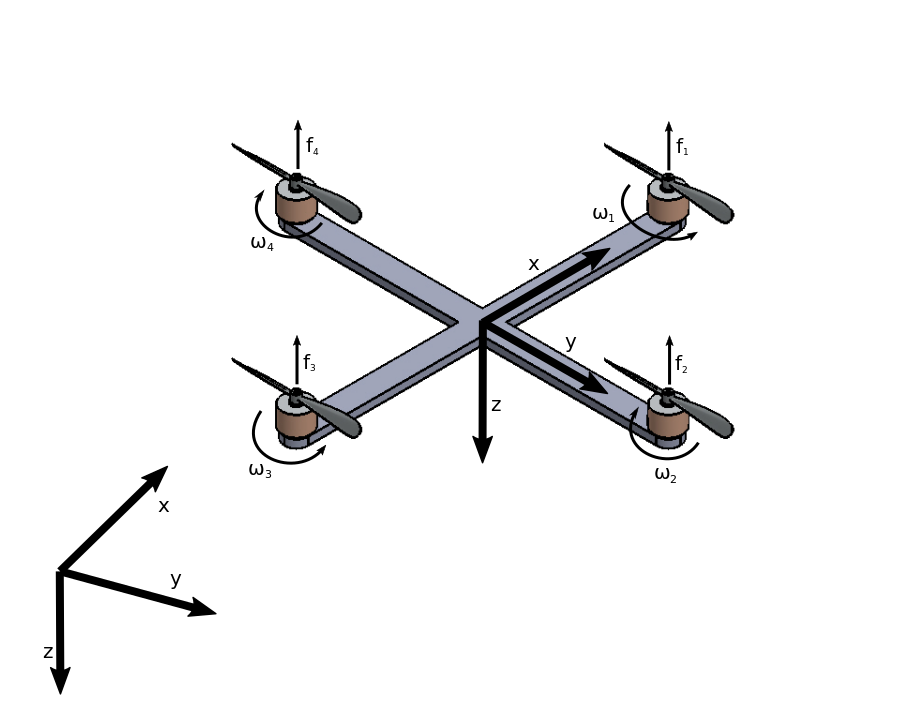
\includegraphics[width=.8\textwidth]{img/simpleQuadRef}
  \caption{Body frame and NED frame}{Illustrates that the position of body-frame is in the center of the UAV. The difference in force from motors one and three generates torque about the body frame y axis, while motor 2 and 4 affects the torque about the x axis. }
  \label{fig:quadRef}
\end{figure}

Angular momentum acting on the UAV frame is generated from the difference in force generated from motors across the x and y axis of the body frame (\cite{lozano2013unmanned}). The difference in force from 
motor one and three gives an angular momentum around the y axis, while difference in force from motor two and four generates angular momentum around the x axis. The relation between angular- and linear moment 
is $\vect{m}=\vect{r}\times \vect{f}$, where $\vect{r}$ is the vector from center of rotation to the linear force, and $\vect{f}$ is the linear moment (\cite{egeland2002modeling}). There is also generated 
angular momentum around the z axis. This momentum are generated due to the drag force from the propellers (\cite{nicolai2001fundamentals}), and can be formulated as $d\vect{\omega}^2_i$, where $d$ is the drag factor and
$\omega_i$ is the angular velocity for propeller $i$. By using the right-hand rule to determine the directions at the forces and momentums, we can summarize the input torques as
\renewcommand*{\arraystretch}{1}
\begin{equation}
  \vect{m}_b^b=
  \begin{bmatrix}
    lk(\vect{\omega}_4^2-\vect{\omega}_2^2)\\
    lk(\vect{\omega}_1^2-\vect{\omega}_3^2)\\
    d(-\vect{\omega}_1+\vect{\omega}_2-\vect{\omega}_3+\vect{\omega}_4)
  \end{bmatrix}
\end{equation}
Where $l$ is the distance from the body frame to the propeller.
%There are allso gyroscopic torques caused by the moments of inertia in the propellars.

By using the angular velocity transformation and the rotation matrix differential equations defined in \ref{sec:euler}, the kinematic equations for the position and attitude can be summarized on the
form $\vect{\dot{\vect{\eta}}}=\vect{J}(\vect{\eta})\vect{\nu}$ as (\cite{Fossen2011})
\begin{equation}\label{eq:rotVelEul}
  \begin{bmatrix}
    \vect{\dot{p}}_{n/b}^n\\
    \vect{\dot{\Theta}}_{nb}\\
  \end{bmatrix}
  =
  \begin{bmatrix}
    \vect{R}_b^n(\vect{\Theta}_nb) & \vect{0}^{3 \times 3}\\
    \vect{0}^{3 \times 3} & \vect{T}_{\Theta}(\vect{\Theta}_nb)
  \end{bmatrix}
  \begin{bmatrix}
    \vect{v}_{b/n}^b\\
    \vect{\omega}_{b/n}^b
  \end{bmatrix}
\end{equation}
The Euler angle approach is used for this equation set. The kinematic equation can also be defined for the singularity free unit quaternions defined in \ref{sec:quat} (Fossen2011)
\begin{equation}\label{eq:rotVelQuat}
  \begin{bmatrix}
    \vect{\dot{p}}_{n/b}^n\\
    \vect{\dot{q}}\\
  \end{bmatrix}
  =
  \begin{bmatrix}
    \vect{R}_b^n(\vect{q}) & \vect{0}^{3 \times 3}\\
    \vect{0}^{4 \times 3} & \vect{T}_{q}(\vect{q})
  \end{bmatrix}
  \begin{bmatrix}
    \vect{v}_{b/n}^b\\
    \vect{\omega}_{b/n}^b
  \end{bmatrix}
\end{equation}
The 12 state differential equation set can be summarized as
\begin{equation}
  \begin{bmatrix}
    \dot{\vect{\nu}}\\
    \dot{\vect{\eta}}
  \end{bmatrix}
  =
  \begin{bmatrix}
    \vect{M}_{RB}^{-1}(\vect{\tau}_{RB}-\vect{C}_{RB}(\vect{\nu})\vect{\nu})\\
    \vect{J}(\vect{\eta})\vect{\nu}
  \end{bmatrix}
\end{equation}
where $\vect{J}$ is either the $\vect{J}_\Theta$ from equation~\ref{eq:rotVelEul} using the Euler method or $\vect{J}_q$ from equation~\ref{eq:rotVelQuat} using quaternions.
%\subsection{Simplified model}

